\documentclass{article}\usepackage[]{graphicx}\usepackage[]{color}
%% maxwidth is the original width if it is less than linewidth
%% otherwise use linewidth (to make sure the graphics do not exceed the margin)
\makeatletter
\def\maxwidth{ %
  \ifdim\Gin@nat@width>\linewidth
    \linewidth
  \else
    \Gin@nat@width
  \fi
}
\makeatother

\definecolor{fgcolor}{rgb}{0.345, 0.345, 0.345}
\newcommand{\hlnum}[1]{\textcolor[rgb]{0.686,0.059,0.569}{#1}}%
\newcommand{\hlstr}[1]{\textcolor[rgb]{0.192,0.494,0.8}{#1}}%
\newcommand{\hlcom}[1]{\textcolor[rgb]{0.678,0.584,0.686}{\textit{#1}}}%
\newcommand{\hlopt}[1]{\textcolor[rgb]{0,0,0}{#1}}%
\newcommand{\hlstd}[1]{\textcolor[rgb]{0.345,0.345,0.345}{#1}}%
\newcommand{\hlkwa}[1]{\textcolor[rgb]{0.161,0.373,0.58}{\textbf{#1}}}%
\newcommand{\hlkwb}[1]{\textcolor[rgb]{0.69,0.353,0.396}{#1}}%
\newcommand{\hlkwc}[1]{\textcolor[rgb]{0.333,0.667,0.333}{#1}}%
\newcommand{\hlkwd}[1]{\textcolor[rgb]{0.737,0.353,0.396}{\textbf{#1}}}%

\usepackage{framed}
\makeatletter
\newenvironment{kframe}{%
 \def\at@end@of@kframe{}%
 \ifinner\ifhmode%
  \def\at@end@of@kframe{\end{minipage}}%
  \begin{minipage}{\columnwidth}%
 \fi\fi%
 \def\FrameCommand##1{\hskip\@totalleftmargin \hskip-\fboxsep
 \colorbox{shadecolor}{##1}\hskip-\fboxsep
     % There is no \\@totalrightmargin, so:
     \hskip-\linewidth \hskip-\@totalleftmargin \hskip\columnwidth}%
 \MakeFramed {\advance\hsize-\width
   \@totalleftmargin\z@ \linewidth\hsize
   \@setminipage}}%
 {\par\unskip\endMakeFramed%
 \at@end@of@kframe}
\makeatother

\definecolor{shadecolor}{rgb}{.97, .97, .97}
\definecolor{messagecolor}{rgb}{0, 0, 0}
\definecolor{warningcolor}{rgb}{1, 0, 1}
\definecolor{errorcolor}{rgb}{1, 0, 0}
\newenvironment{knitrout}{}{} % an empty environment to be redefined in TeX

\usepackage{alltt}
\setlength\parindent{0pt}
\usepackage{mdframed}
\IfFileExists{upquote.sty}{\usepackage{upquote}}{}
\begin{document}



\begin{mdframed}
\textbf{Please note:} in this analysis I consider \texttt{phi} to describe the state of the individual as we counted it. If \texttt{phi[i,t]} is $0$ it means that the individual is found back dead and is thus not part of the alive population. It has to be noted anyway that not all data is updated when an individual dies. The last entry of an individual with \texttt{phi==1} will have the same values for at least \texttt{Z,ARS, AGE} as the entry where the individual was encountered dead (\texttt{phi==0}). So far I focus on females only.
\end{mdframed}
\begin{knitrout}
\definecolor{shadecolor}{rgb}{0.969, 0.969, 0.969}\color{fgcolor}\begin{kframe}
\begin{alltt}
\hlstd{dat}\hlkwb{<-}\hlkwd{read.table}\hlstd{(}\hlkwc{file}\hlstd{=}\hlstr{"pop.csv"}\hlstd{,}\hlkwc{header}\hlstd{=T)}
\hlkwd{head}\hlstd{(dat,}\hlnum{5}\hlstd{)}
\end{alltt}
\begin{verbatim}
##   t ID     z     bvs    C s ARS age p1 p2 phi
## 1 1  2 11.61  0.8402  249 M   0   1 NA NA   1
## 2 1  3 13.14  1.0114  587 F  26   1 NA NA   1
## 3 1  4 13.71  0.2694 2427 M   0   1 NA NA   1
## 4 1  5 10.88 -0.9088   89 F   5   1 NA NA   1
## 5 1  8 10.94  0.2045   85 F   7   1 NA NA   1
\end{verbatim}
\begin{alltt}
\hlkwd{which}\hlstd{(}\hlopt{!}\hlstd{(}\hlkwd{min}\hlstd{(dat}\hlopt{$}\hlstd{ID)}\hlopt{:}\hlkwd{max}\hlstd{(dat}\hlopt{$}\hlstd{ID)}\hlopt\hlstd{dat}\hlopt{$}\hlstd{ID))}
\end{alltt}
\begin{verbatim}
## integer(0)
\end{verbatim}
\end{kframe}
\end{knitrout}


\begin{knitrout}
\definecolor{shadecolor}{rgb}{0.969, 0.969, 0.969}\color{fgcolor}\begin{kframe}
\begin{alltt}
\hlstd{dat2}\hlkwb{<-}\hlkwd{subset}\hlstd{(dat,phi}\hlopt{==}\hlnum{1}\hlstd{)}
\hlstd{dat2}\hlkwb{<-}\hlstd{dat2[,}\hlkwd{c}\hlstd{(}\hlstr{"ID"}\hlstd{,}\hlstr{"t"}\hlstd{,}\hlstr{"z"}\hlstd{)]}
\hlkwd{library}\hlstd{(}\hlstr{'reshape'}\hlstd{)}
\end{alltt}


{\ttfamily\noindent\itshape\color{messagecolor}{\#\# Loading required package: plyr\\\#\# \\\#\# Attaching package: 'reshape'\\\#\# \\\#\# The following objects are masked from 'package:plyr':\\\#\# \\\#\#\ \ \ \  rename, round\_any}}\begin{alltt}
\hlkwd{par}\hlstd{(}\hlkwc{mar}\hlstd{=}\hlkwd{c}\hlstd{(}\hlnum{6}\hlstd{,}\hlnum{6}\hlstd{,}\hlnum{2}\hlstd{,}\hlnum{2}\hlstd{))}
\hlstd{dat3}\hlkwb{<-}\hlkwd{reshape}\hlstd{(dat2,} \hlkwc{idvar} \hlstd{=} \hlstr{"ID"}\hlstd{,} \hlkwc{timevar} \hlstd{=} \hlstr{"t"}\hlstd{,} \hlkwc{direction} \hlstd{=} \hlstr{"wide"}\hlstd{)}
\hlkwa{for}\hlstd{(i} \hlkwa{in} \hlnum{2}\hlopt{:}\hlstd{(}\hlkwd{ncol}\hlstd{(dat3)}\hlopt{-}\hlnum{2}\hlstd{))\{}
  \hlkwd{plot}\hlstd{(dat3[,i],dat3[,i}\hlopt{+}\hlnum{1}\hlstd{],}\hlkwc{main}\hlstd{=}\hlkwd{paste}\hlstd{(}\hlstr{"Year"}\hlstd{,i}\hlopt{-}\hlnum{1}\hlstd{),}\hlkwc{xlab}\hlstd{=}\hlkwd{paste}\hlstd{(}\hlstr{"z("}\hlstd{,i}\hlopt{-}\hlnum{1}\hlstd{,}\hlstr{")"}\hlstd{,}\hlkwc{sep}\hlstd{=}\hlstr{""}\hlstd{),}\hlkwc{ylab}\hlstd{=}\hlkwd{paste}\hlstd{(}\hlstr{"z("}\hlstd{,i,}\hlstr{")"}\hlstd{,}\hlkwc{sep}\hlstd{=}\hlstr{""}\hlstd{))}
\hlstd{\}}
\hlcom{#temp<-dat[,-c("t","z")]}
\hlcom{#temp<-temp[!duplicated(temp),]}
\hlcom{#dat4<-merge(dat3,temp,by="ID")}
\hlcom{#dat4}
\end{alltt}
\end{kframe}
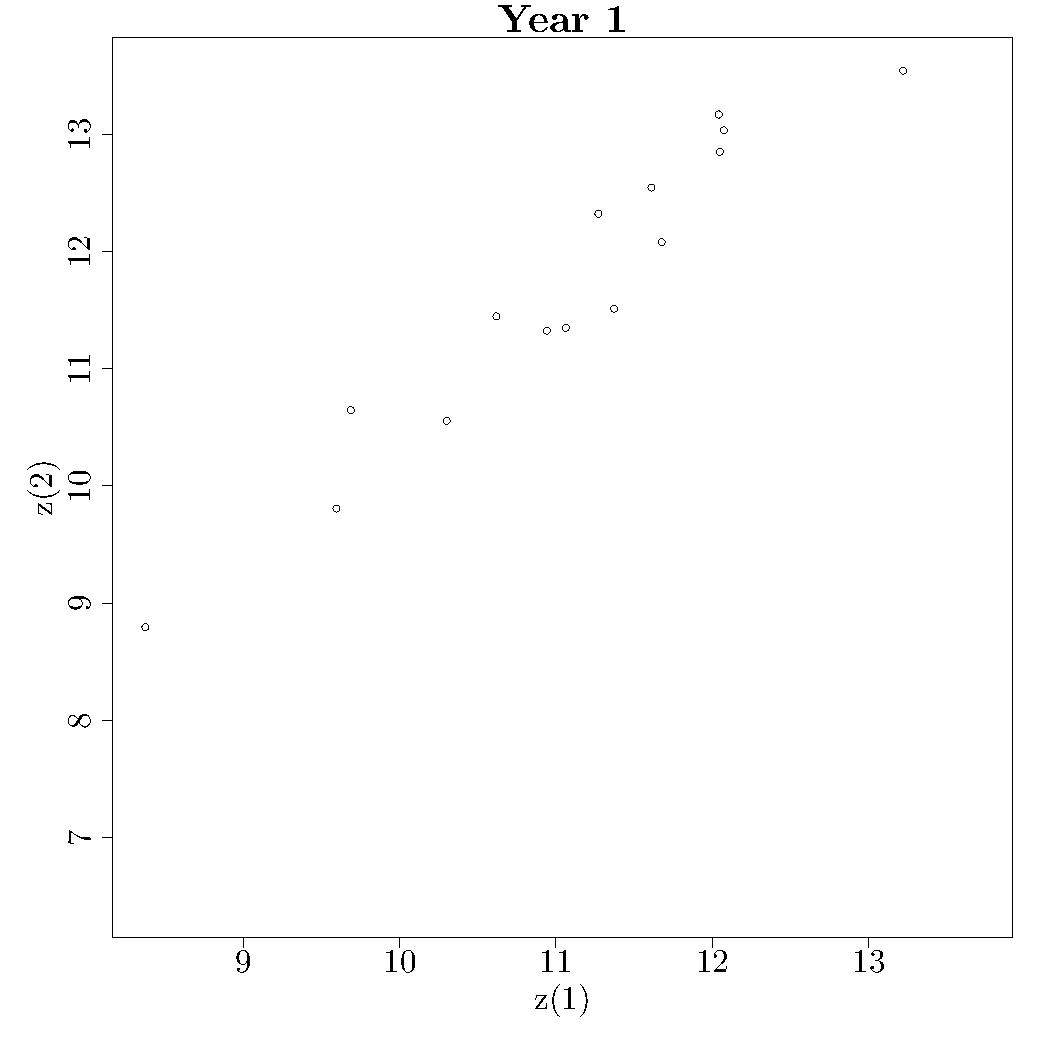
\includegraphics[width=0.35\textwidth]{figure/Reshaping1} 
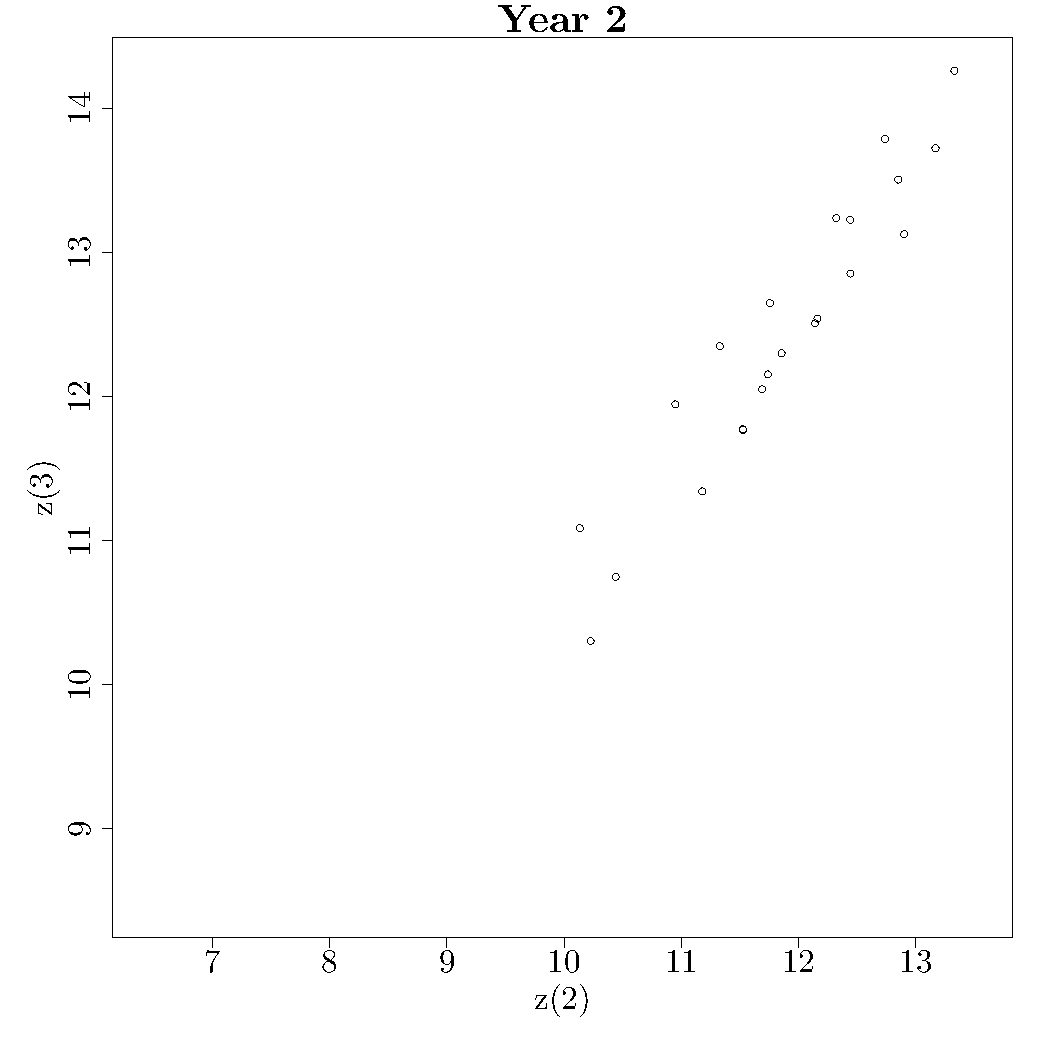
\includegraphics[width=0.35\textwidth]{figure/Reshaping2} 
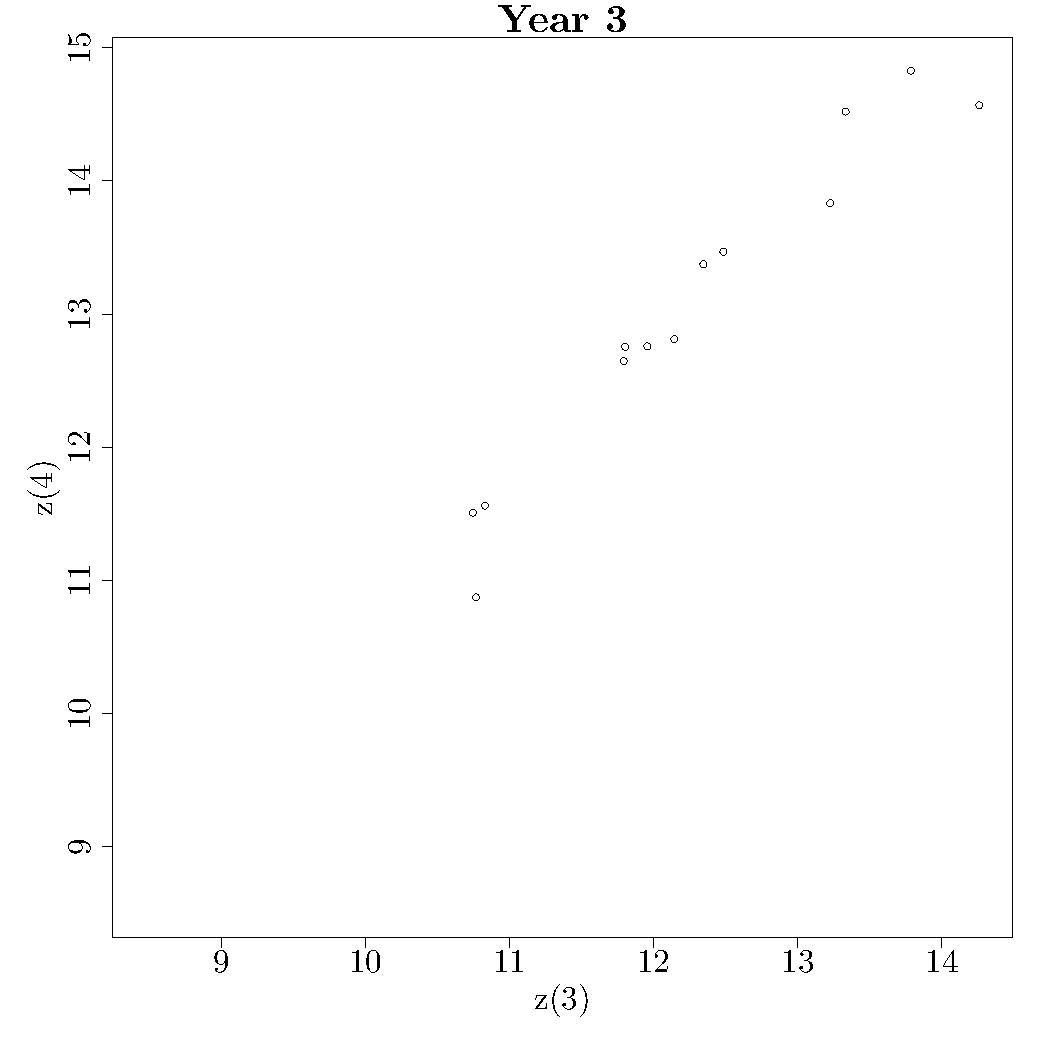
\includegraphics[width=0.35\textwidth]{figure/Reshaping3} 
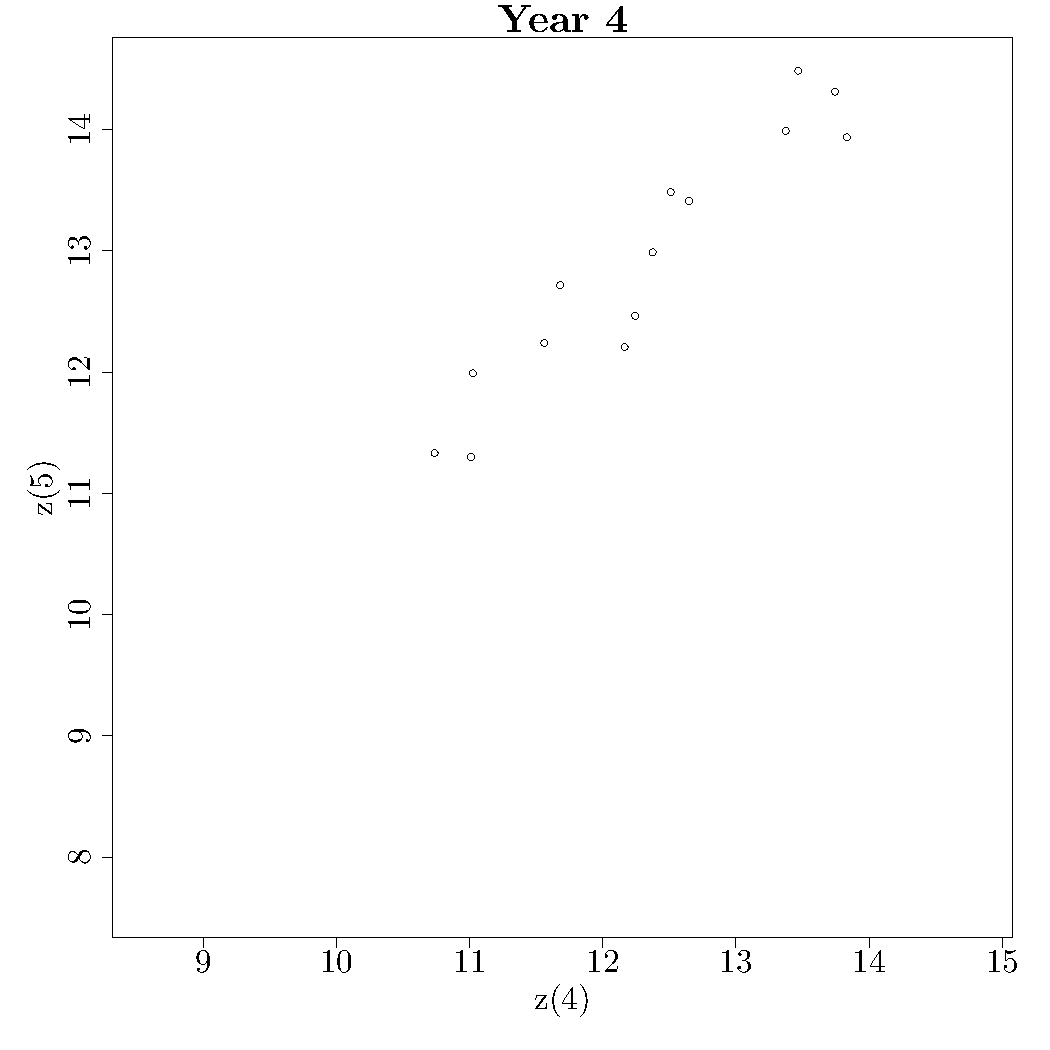
\includegraphics[width=0.35\textwidth]{figure/Reshaping4} 
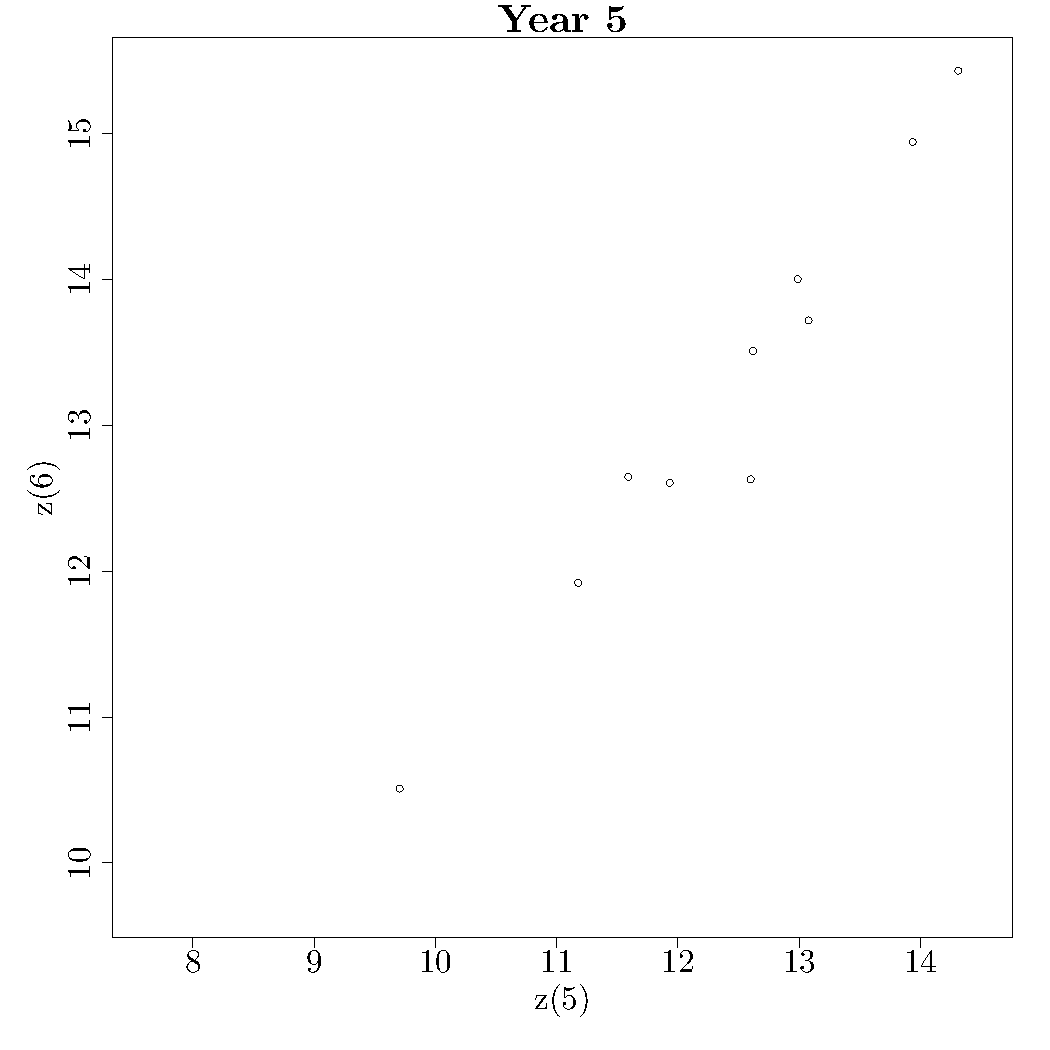
\includegraphics[width=0.35\textwidth]{figure/Reshaping5} 
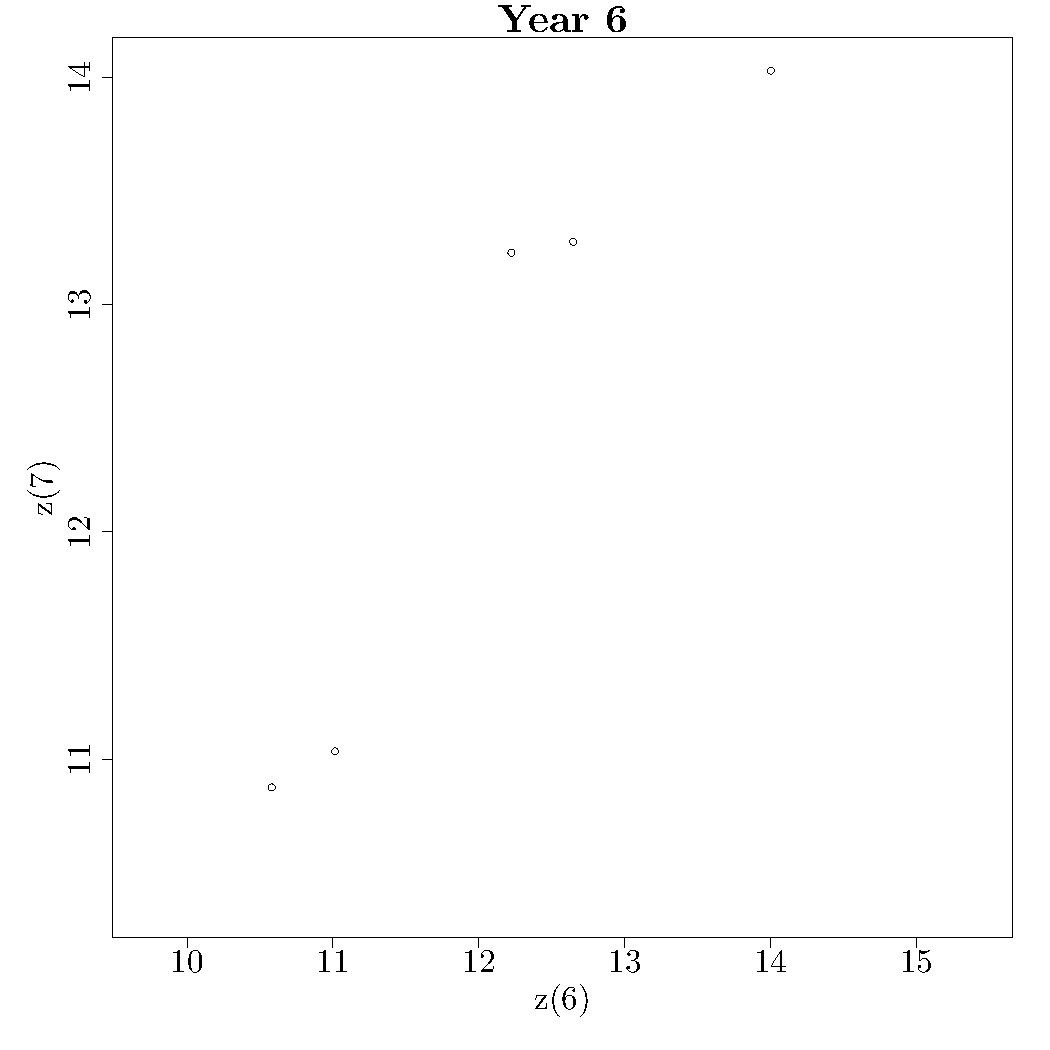
\includegraphics[width=0.35\textwidth]{figure/Reshaping6} 
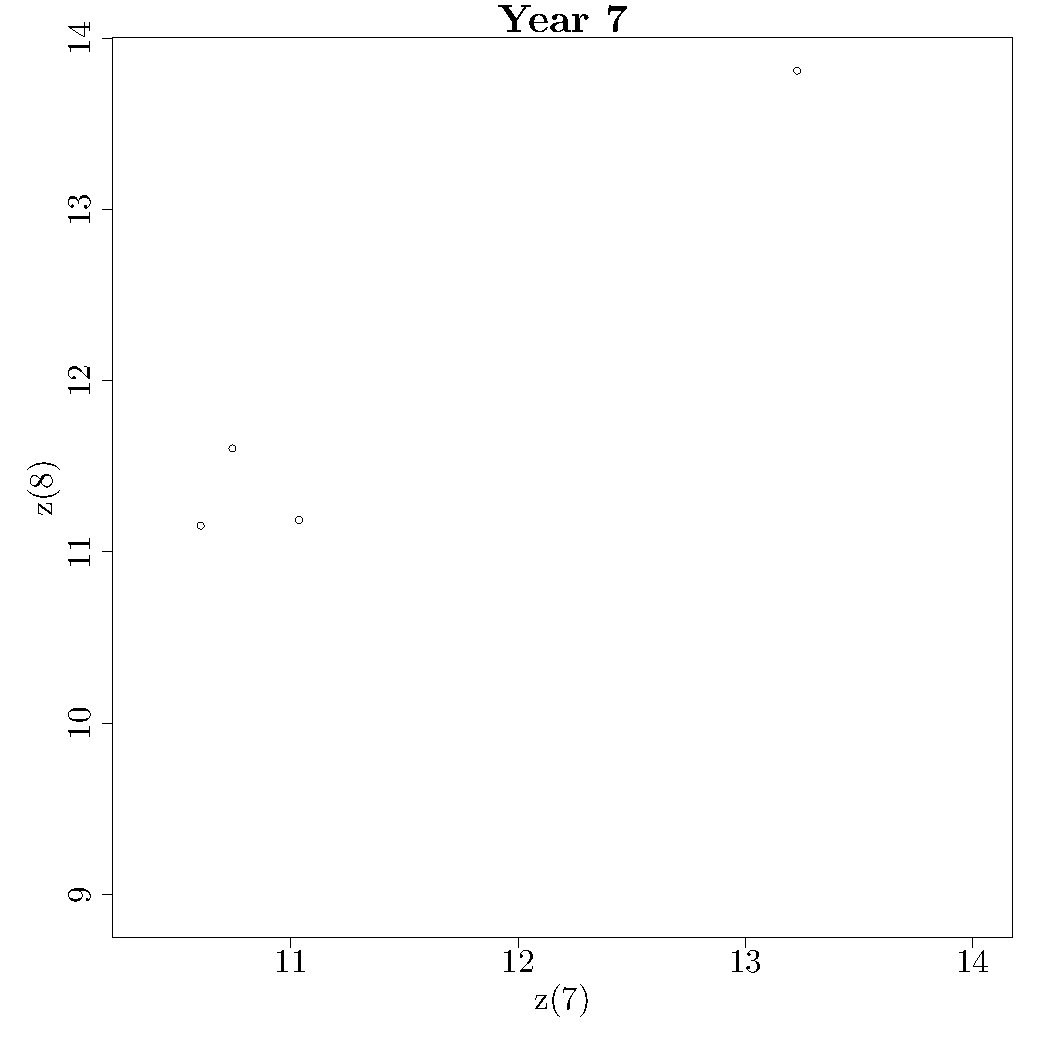
\includegraphics[width=0.35\textwidth]{figure/Reshaping7} 
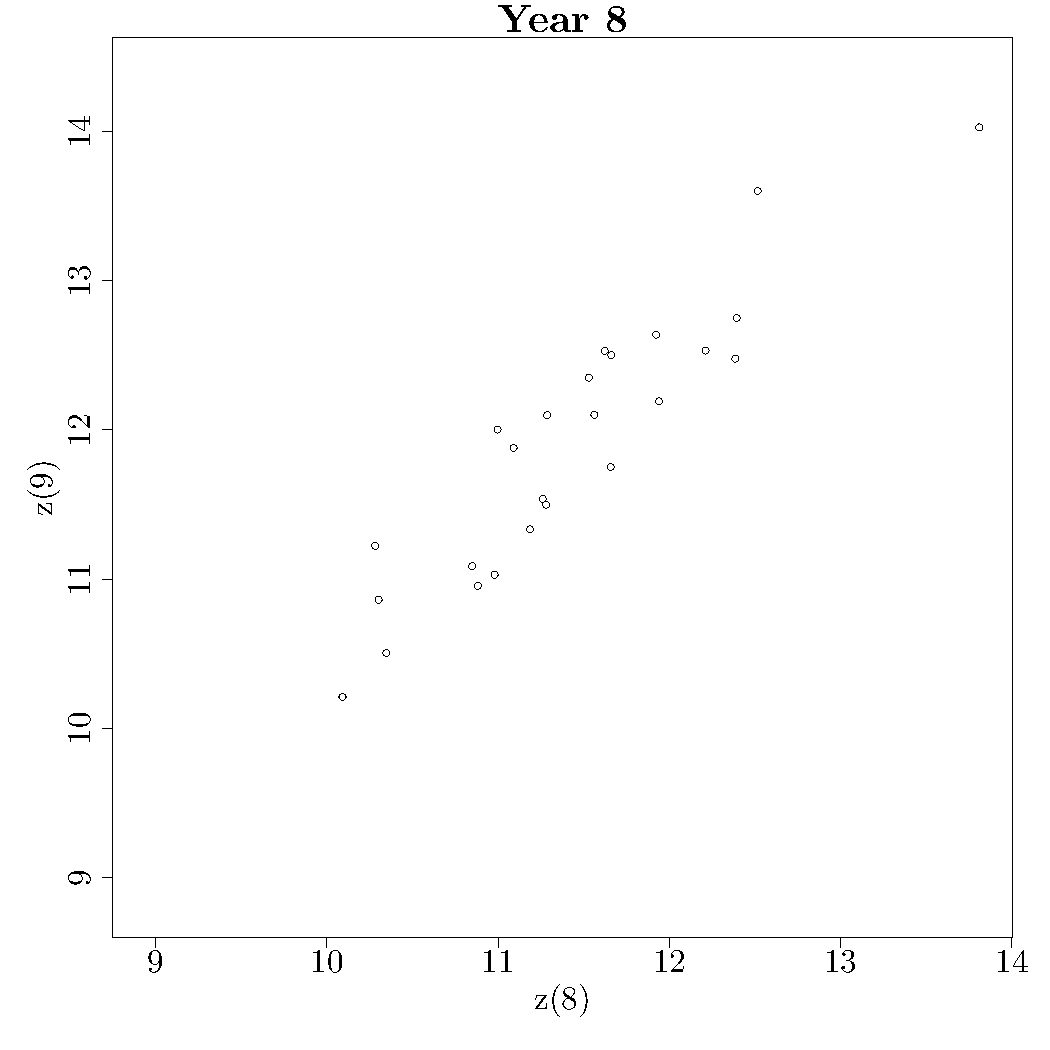
\includegraphics[width=0.35\textwidth]{figure/Reshaping8} 
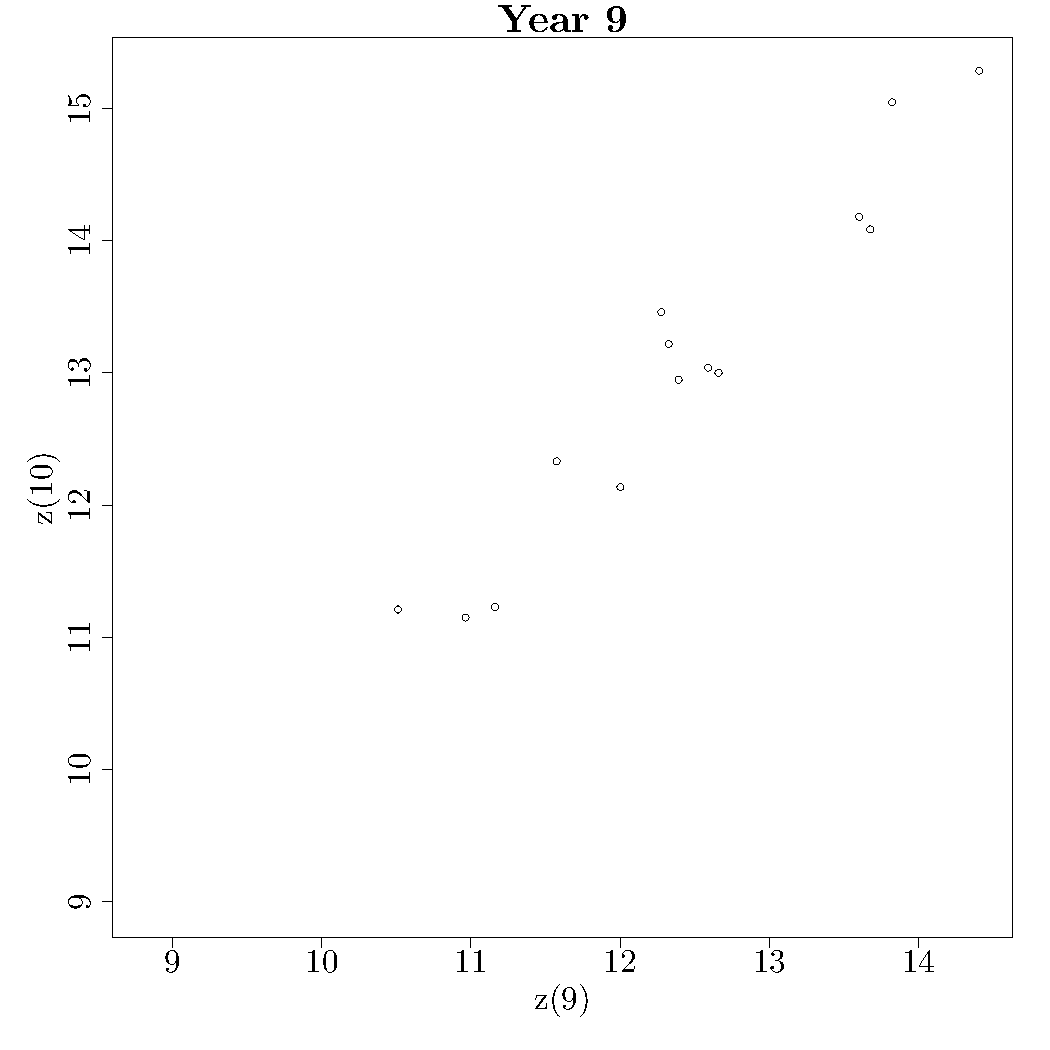
\includegraphics[width=0.35\textwidth]{figure/Reshaping9} 
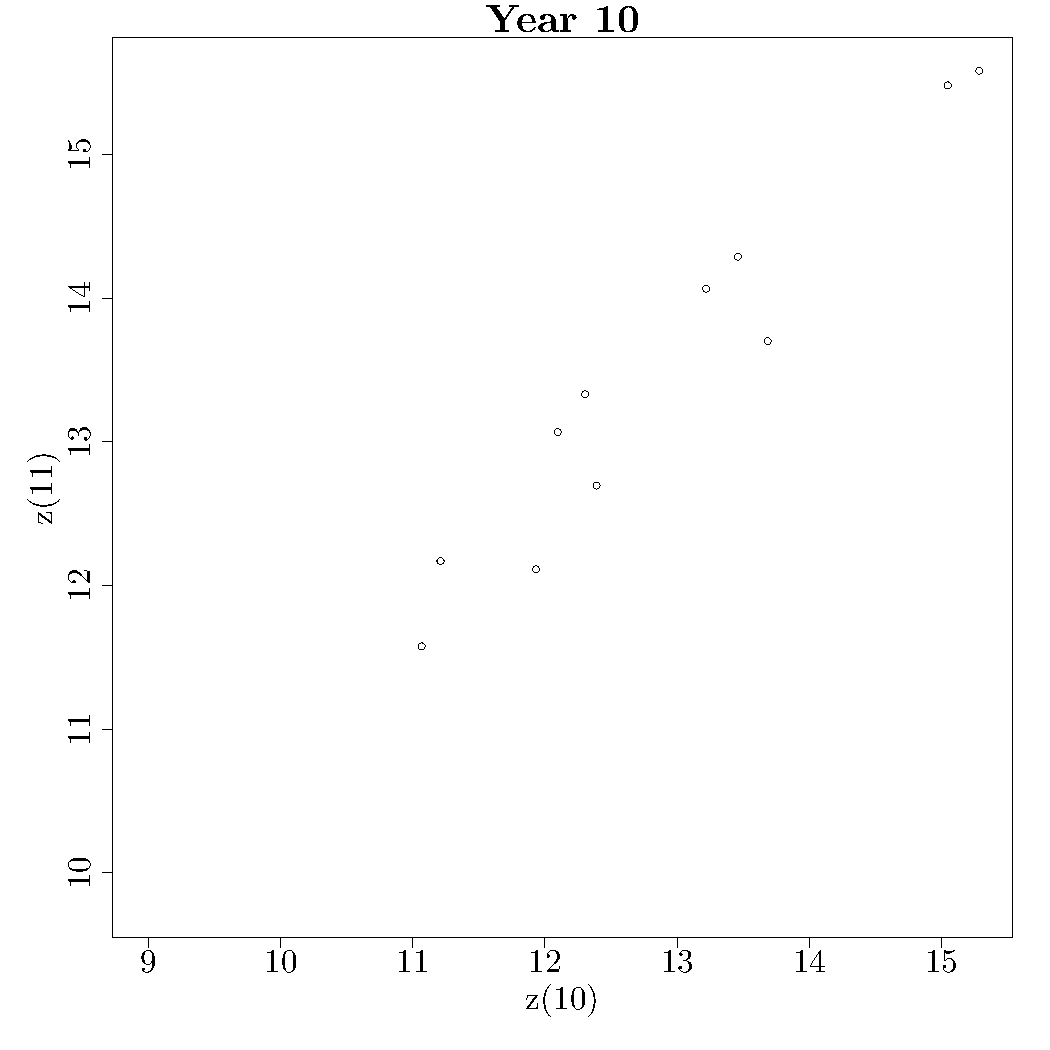
\includegraphics[width=0.35\textwidth]{figure/Reshaping10} 
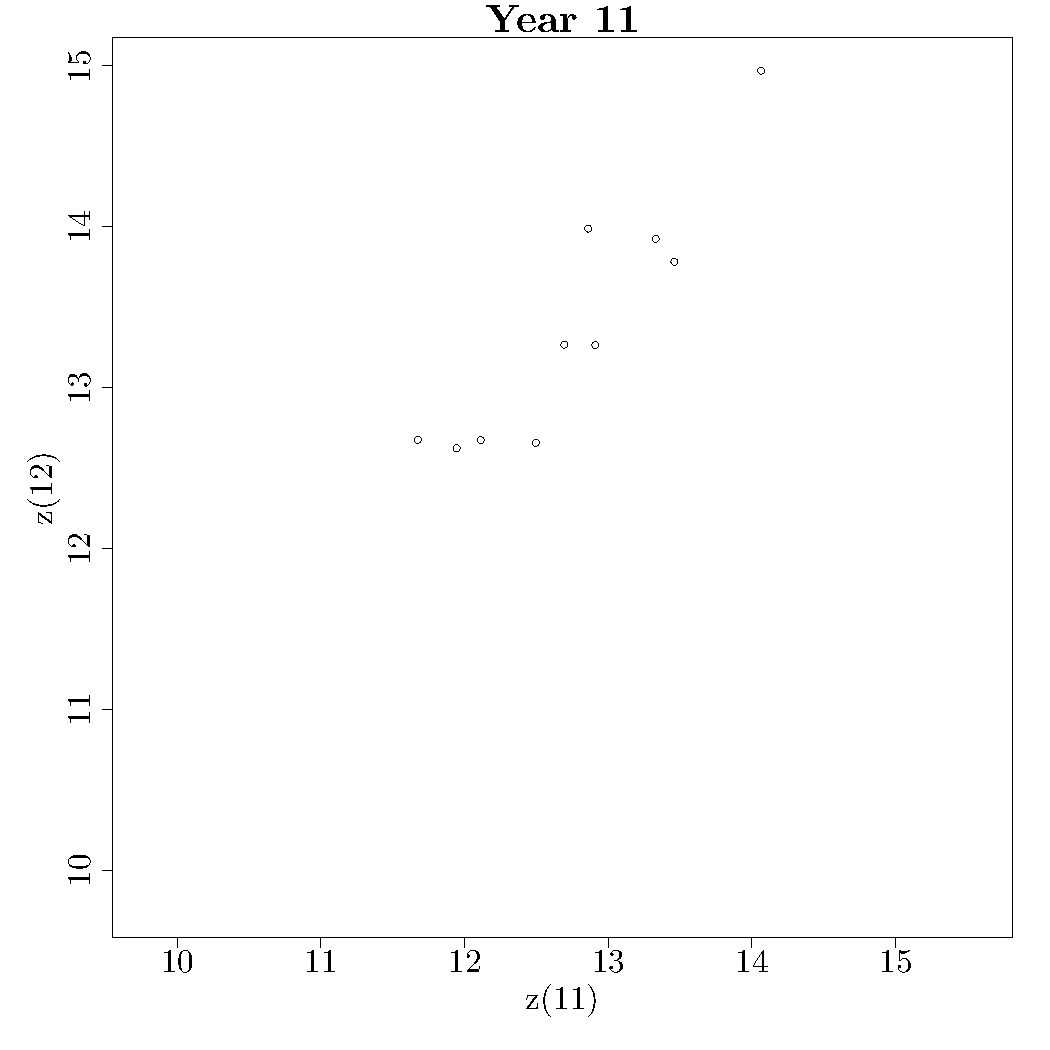
\includegraphics[width=0.35\textwidth]{figure/Reshaping11} 
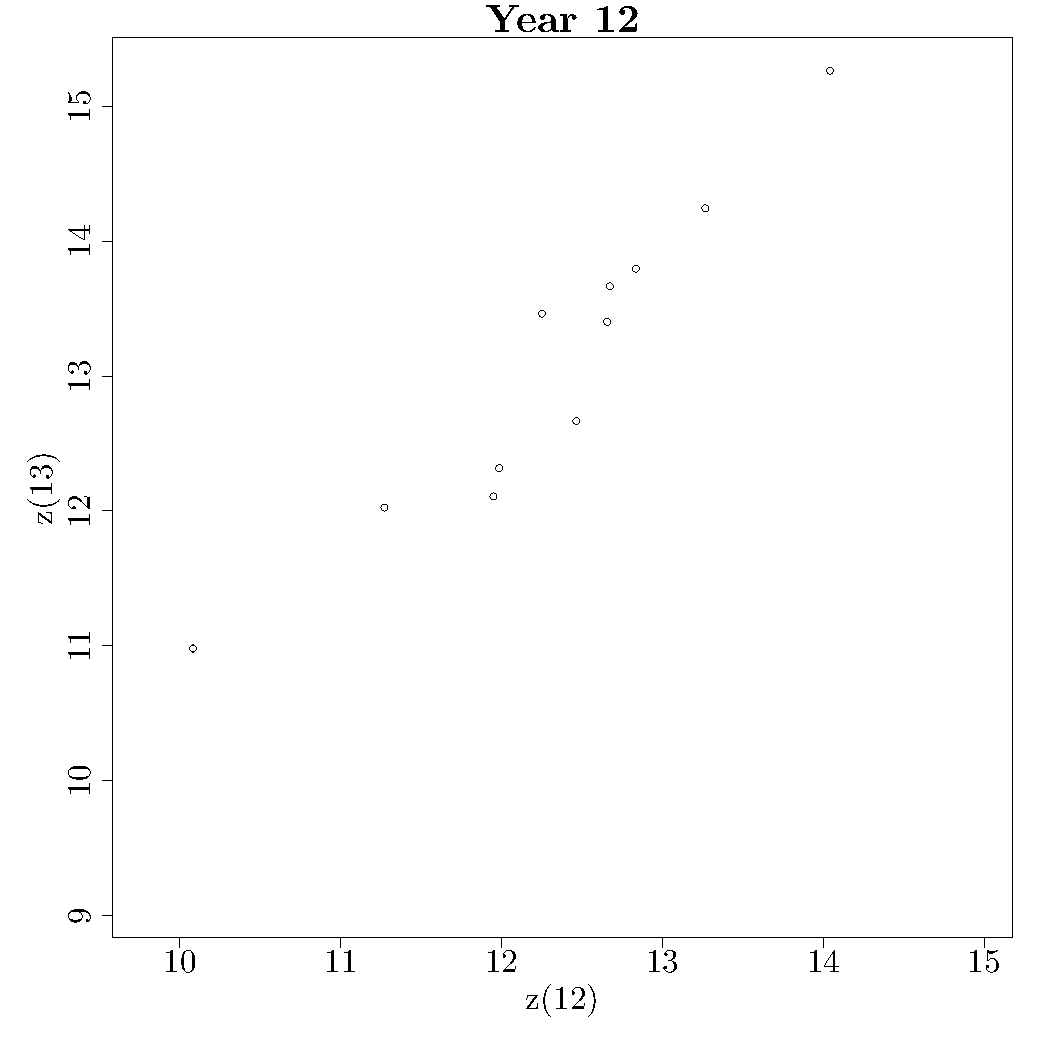
\includegraphics[width=0.35\textwidth]{figure/Reshaping12} 
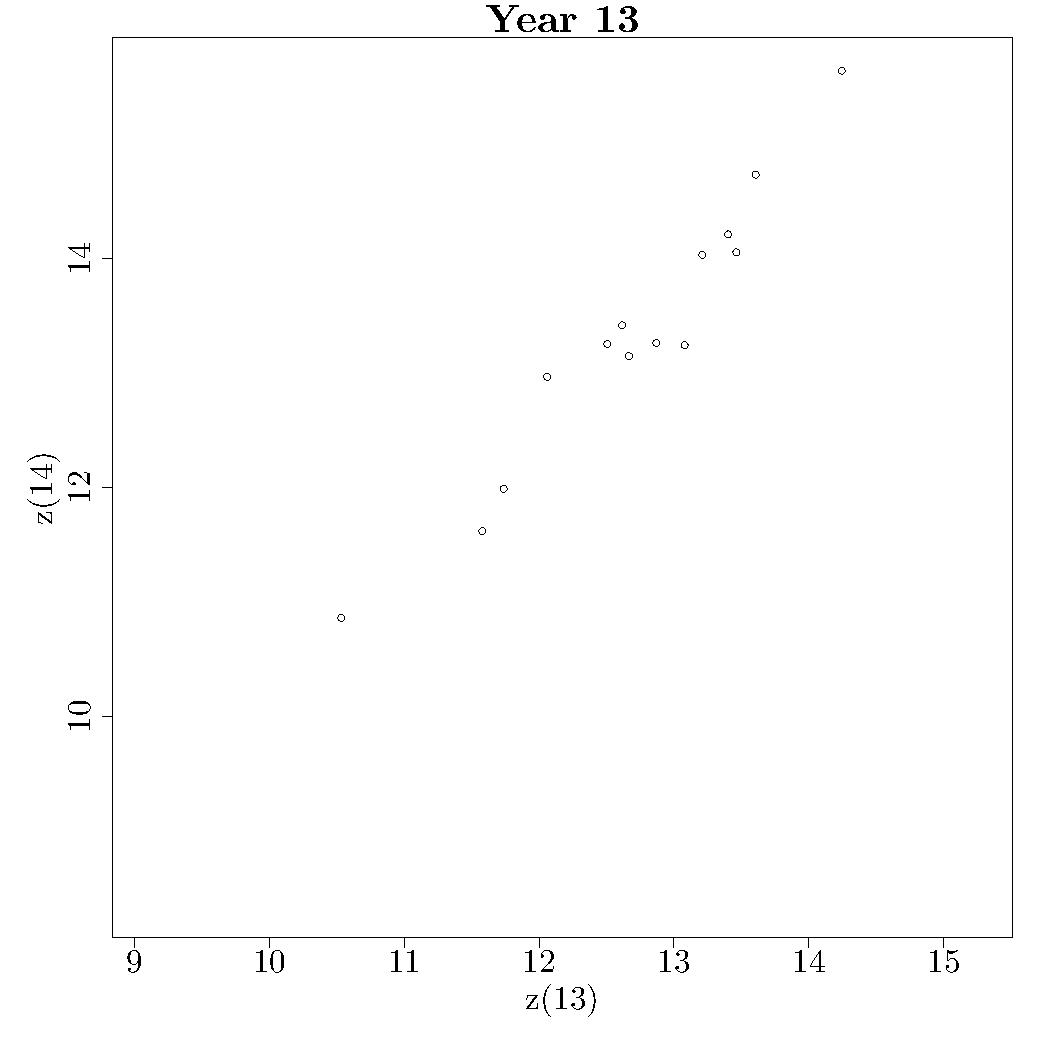
\includegraphics[width=0.35\textwidth]{figure/Reshaping13} 
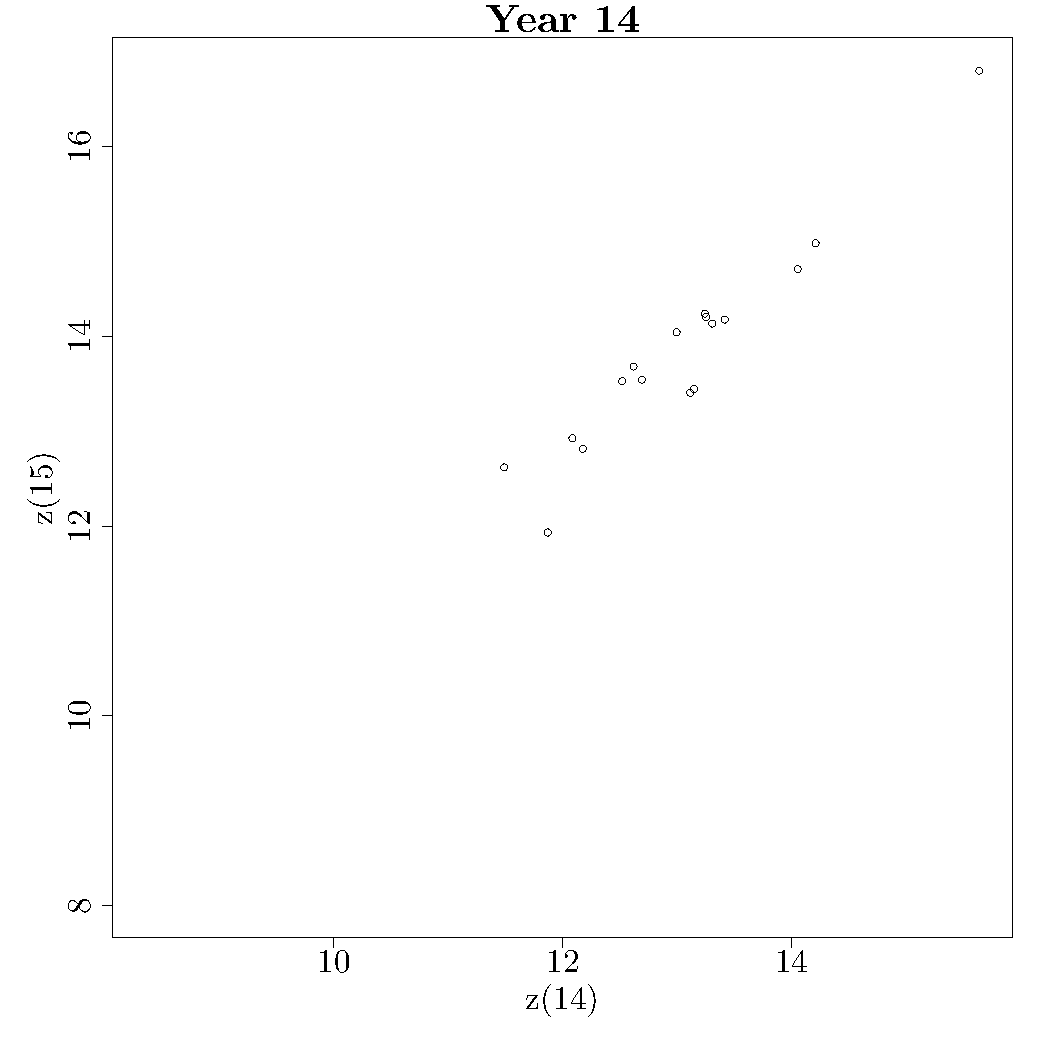
\includegraphics[width=0.35\textwidth]{figure/Reshaping14} 
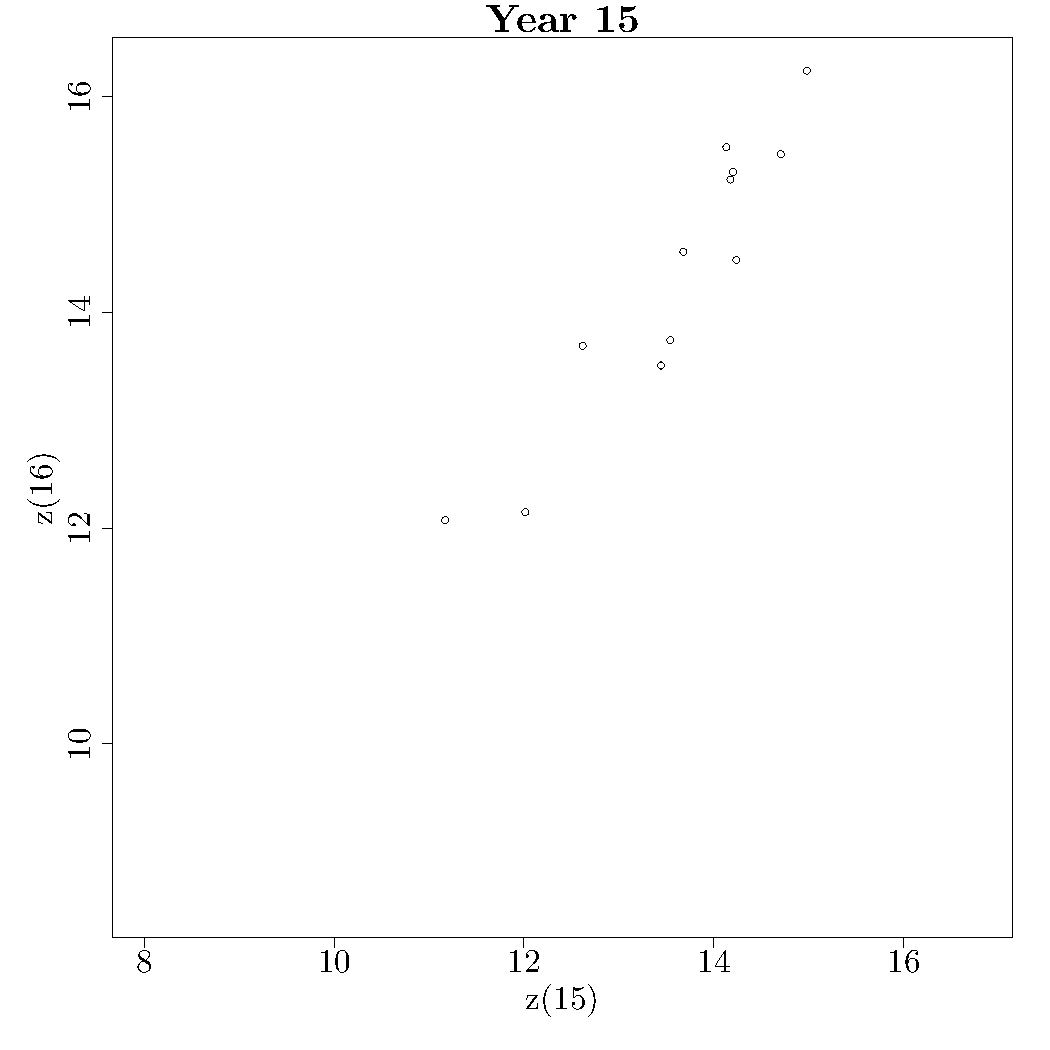
\includegraphics[width=0.35\textwidth]{figure/Reshaping15} 
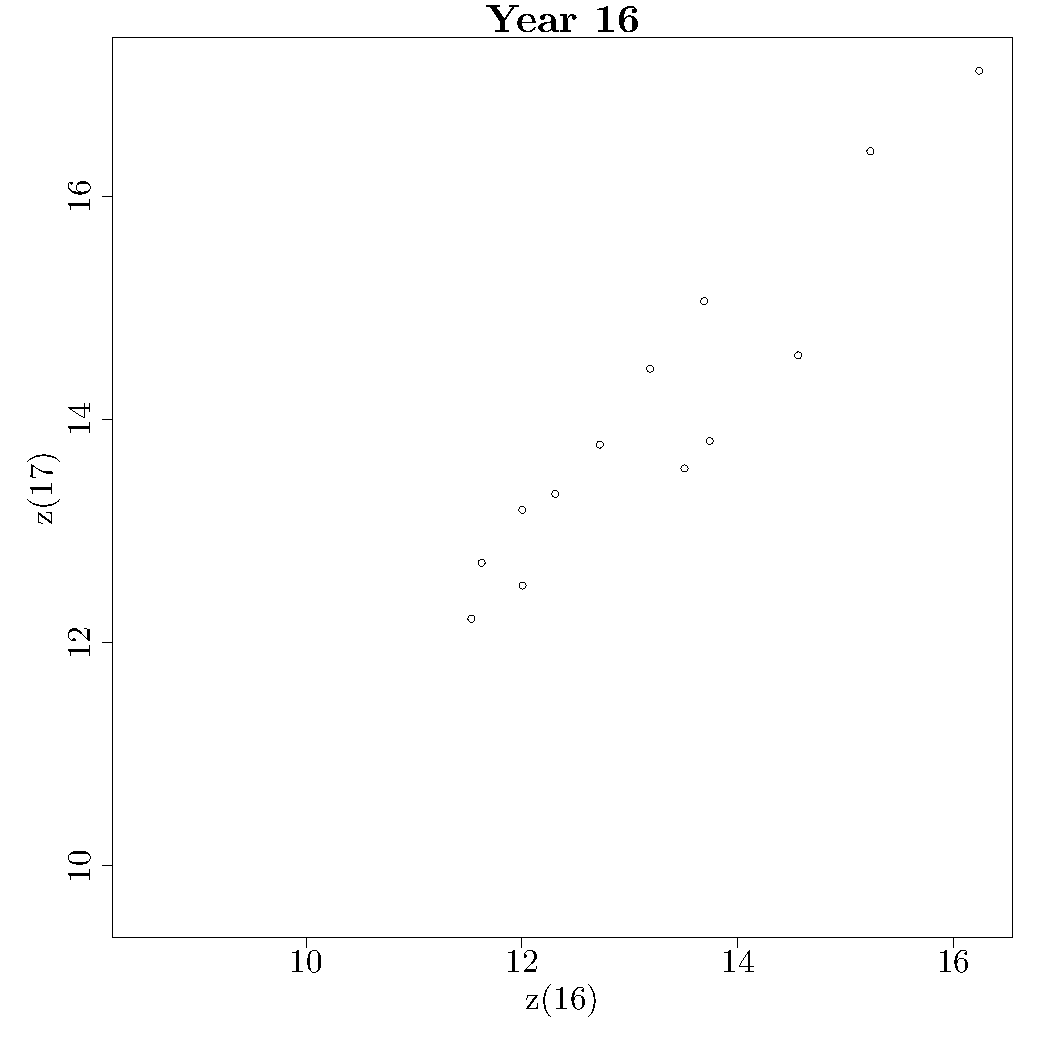
\includegraphics[width=0.35\textwidth]{figure/Reshaping16} 
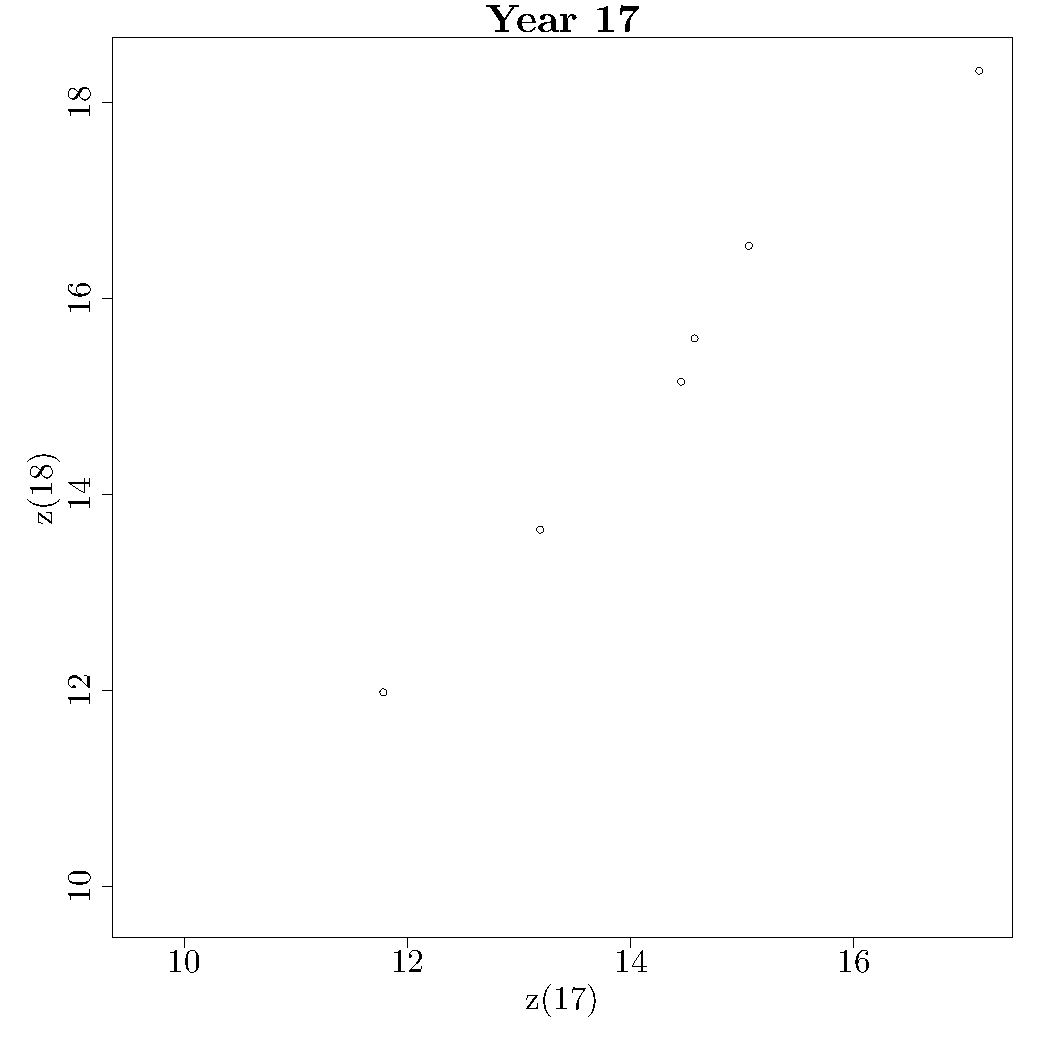
\includegraphics[width=0.35\textwidth]{figure/Reshaping17} 

\end{knitrout}

Let us first take a look how the average body mass in the population (in this preliminary analysis we discard all information on age structure, I will include this later.) I also calculate average offspring trait values and the number of female offspring per individual.
\begin{knitrout}
\definecolor{shadecolor}{rgb}{0.969, 0.969, 0.969}\color{fgcolor}\begin{kframe}
\begin{alltt}
\hlkwd{par}\hlstd{(}\hlkwc{mar}\hlstd{=}\hlkwd{c}\hlstd{(}\hlnum{6}\hlstd{,}\hlnum{6}\hlstd{,}\hlnum{2}\hlstd{,}\hlnum{2}\hlstd{))}
\hlstd{alive}\hlkwb{<-}\hlkwd{subset}\hlstd{(dat,phi}\hlopt{==}\hlnum{1} \hlopt{&} \hlstd{s}\hlopt{==}\hlstr{'F'}\hlstd{)} \hlcom{# We take only the alive individuals}
\hlstd{alive}\hlopt{$}\hlstd{zoffs}\hlkwb{<-}\hlnum{NA}
\hlstd{alive}\hlopt{$}\hlstd{g}\hlkwb{<-}\hlnum{0}
\hlstd{alive}\hlopt{$}\hlstd{su}\hlkwb{<-}\hlnum{0}
\hlkwa{for}\hlstd{(i} \hlkwa{in} \hlnum{1}\hlopt{:}\hlkwd{length}\hlstd{(alive}\hlopt{$}\hlstd{t))\{}
  \hlstd{vals}\hlkwb{<-}\hlstd{alive}\hlopt{$}\hlstd{z[(alive}\hlopt{$}\hlstd{p1}\hlopt{==}\hlstd{alive}\hlopt{$}\hlstd{ID[i]} \hlopt{&} \hlstd{alive}\hlopt{$}\hlstd{age}\hlopt{==}\hlnum{0} \hlopt{&} \hlstd{alive}\hlopt{$}\hlstd{t}\hlopt{==}\hlstd{(alive}\hlopt{$}\hlstd{t[i])}\hlopt{+}\hlnum{1}\hlstd{)]}
  \hlstd{alive}\hlopt{$}\hlstd{zoffs[i]}\hlkwb{<-}\hlkwd{mean}\hlstd{(vals,}\hlkwc{na.rm}\hlstd{=T)}
  \hlstd{alive}\hlopt{$}\hlstd{offs[i]}\hlkwb{<-}\hlkwd{length}\hlstd{(vals[}\hlopt{!}\hlkwd{is.na}\hlstd{(vals)])}
  \hlkwa{if}\hlstd{(}\hlkwd{sum}\hlstd{(alive}\hlopt{$}\hlstd{ID}\hlopt{==}\hlstd{alive}\hlopt{$}\hlstd{ID[i]} \hlopt{&} \hlstd{alive}\hlopt{$}\hlstd{t}\hlopt{==}\hlstd{(alive}\hlopt{$}\hlstd{t[i]}\hlopt{+}\hlnum{1}\hlstd{)))\{}
    \hlstd{alive}\hlopt{$}\hlstd{su[i]}\hlkwb{<-}\hlnum{1}
    \hlstd{alive}\hlopt{$}\hlstd{g[i]}\hlkwb{<-}\hlstd{alive}\hlopt{$}\hlstd{z[alive}\hlopt{$}\hlstd{ID}\hlopt{==}\hlstd{alive}\hlopt{$}\hlstd{ID[i]} \hlopt{&} \hlstd{alive}\hlopt{$}\hlstd{t}\hlopt{==}\hlstd{(alive}\hlopt{$}\hlstd{t[i]}\hlopt{+}\hlnum{1}\hlstd{)]}\hlopt{-}\hlstd{alive}\hlopt{$}\hlstd{z[i]}
  \hlstd{\}}

\hlstd{\}}
\hlstd{alive}\hlopt{$}\hlstd{D}\hlkwb{<-}\hlstd{alive}\hlopt{$}\hlstd{zoffs}\hlopt{-}\hlstd{alive}\hlopt{$}\hlstd{z}
\hlstd{alive}\hlopt{$}\hlstd{D[}\hlkwd{is.na}\hlstd{(alive}\hlopt{$}\hlstd{D)]}\hlkwb{<-}\hlnum{0}
\hlstd{means}\hlkwb{<-}\hlkwd{aggregate}\hlstd{(alive}\hlopt{$}\hlstd{z,}\hlkwc{by}\hlstd{=}\hlkwd{list}\hlstd{(alive}\hlopt{$}\hlstd{t),mean)}
\hlkwd{plot}\hlstd{(means[,}\hlnum{1}\hlstd{],means[,}\hlnum{2}\hlstd{],}\hlkwc{type}\hlstd{=}\hlstr{"l"}\hlstd{,}\hlkwc{xlab}\hlstd{=}\hlstr{"t"}\hlstd{,}\hlkwc{ylab}\hlstd{=}\hlstr{"$\textbackslash{}\textbackslash{}overline\{Z\}$"}\hlstd{)}
\end{alltt}
\end{kframe}
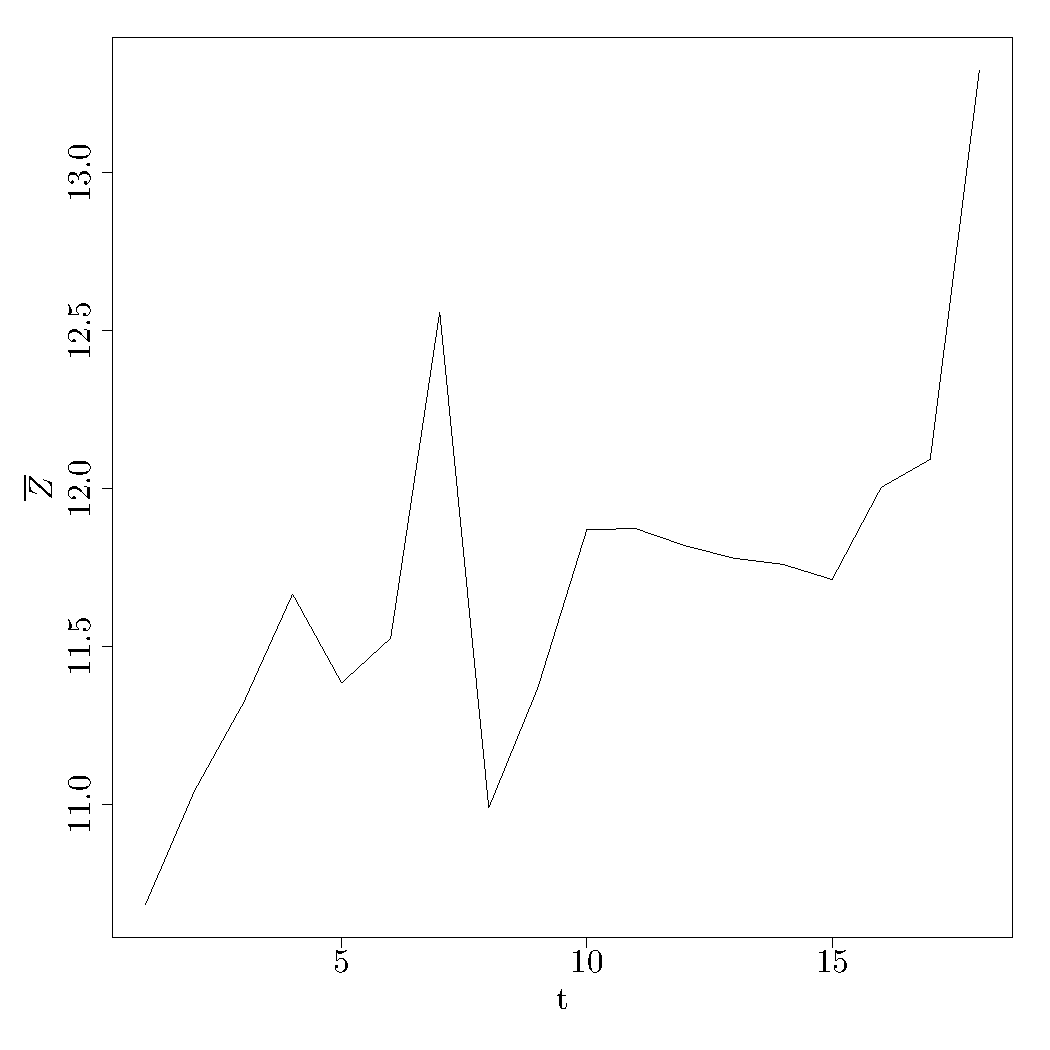
\includegraphics[width=0.75\textwidth]{figure/bodymass_over_years1} 
\begin{kframe}\begin{alltt}
\hlstd{range}\hlkwb{<-}\hlnum{1}\hlopt{:}\hlstd{(}\hlkwd{length}\hlstd{(means[,}\hlnum{1}\hlstd{])}\hlopt{-}\hlnum{1}\hlstd{)}
\hlkwd{plot}\hlstd{(means[range,}\hlnum{1}\hlstd{],means[(range}\hlopt{+}\hlnum{1}\hlstd{),}\hlnum{2}\hlstd{]}\hlopt{-}\hlstd{means[range,}\hlnum{2}\hlstd{],}\hlkwc{type}\hlstd{=}\hlstr{"l"}\hlstd{,}\hlkwc{ylab}\hlstd{=}\hlstr{"$\textbackslash{}\textbackslash{}Delta \textbackslash{}\textbackslash{}overline\{Z\}$"}\hlstd{,}\hlkwc{xlab}\hlstd{=}\hlstr{"t"}\hlstd{)}
\hlkwd{abline}\hlstd{(}\hlkwc{h}\hlstd{=}\hlnum{0}\hlstd{,}\hlkwc{col}\hlstd{=}\hlstr{"gray"}\hlstd{)}
\end{alltt}
\end{kframe}
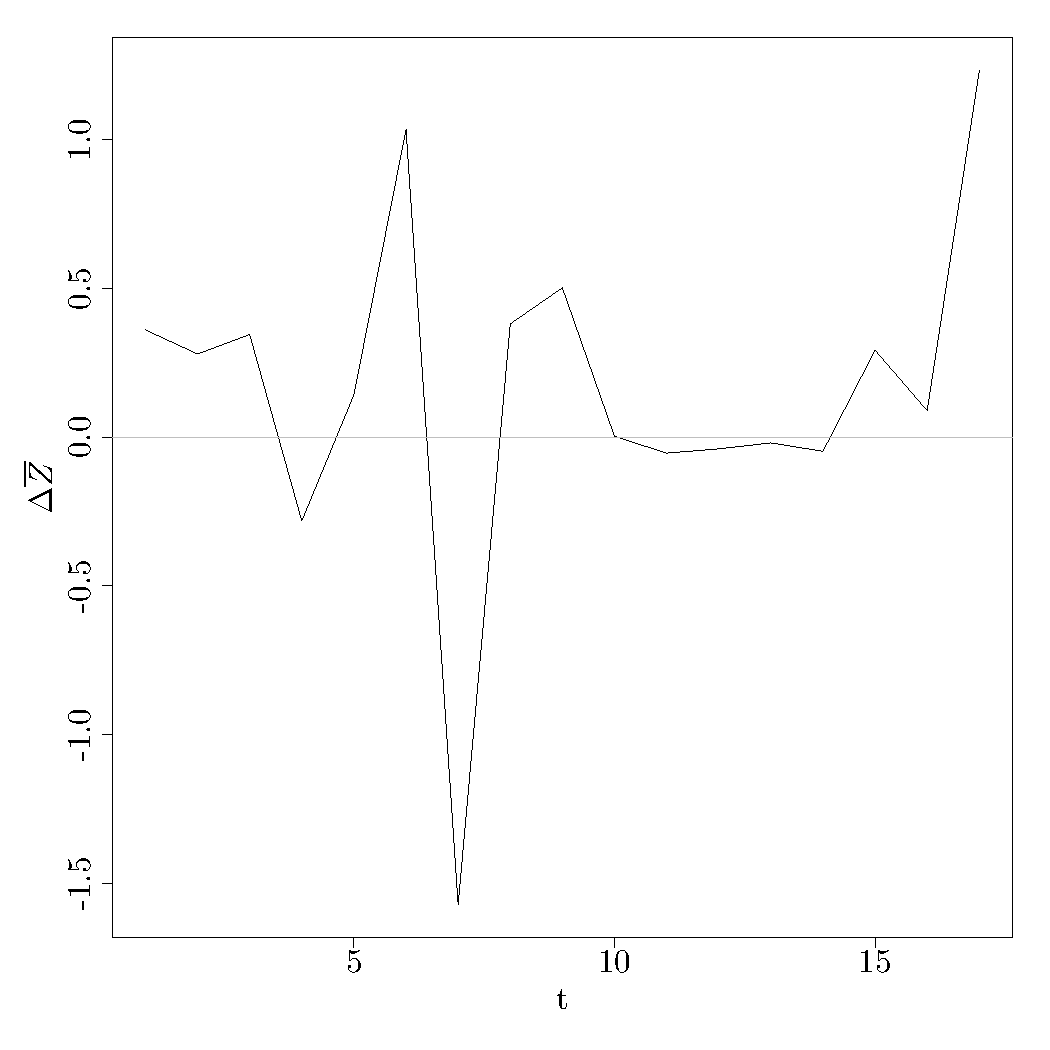
\includegraphics[width=0.75\textwidth]{figure/bodymass_over_years2} 

\end{knitrout}

Now the question is what influences the changes in $\overline{Z}$ over time, is this plasticity, evolution or demography? For this we have to analyse the transitions between two consecutive timesteps.

In order to do so, I first define a new covariance function (that divides by $N$ rather than $N-1$, as we discussed before. I do assume there to be no \texttt{NA}s in the datset, which should be the case for our made up dataset):
\begin{knitrout}
\definecolor{shadecolor}{rgb}{0.969, 0.969, 0.969}\color{fgcolor}\begin{kframe}
\begin{alltt}
\hlstd{mycov}\hlkwb{<-}\hlkwa{function}\hlstd{(}\hlkwc{x}\hlstd{,}\hlkwc{y}\hlstd{)\{}
  \hlkwd{mean}\hlstd{(x}\hlopt{*}\hlstd{y)}\hlopt{-}\hlkwd{mean}\hlstd{(x)}\hlopt{*}\hlkwd{mean}\hlstd{(y)}
\hlstd{\}}
\end{alltt}
\end{kframe}
\end{knitrout}

Now we calculate the actual values:
\begin{knitrout}
\definecolor{shadecolor}{rgb}{0.969, 0.969, 0.969}\color{fgcolor}\begin{kframe}
\begin{alltt}
\hlstd{from}\hlkwb{<-}\hlkwd{min}\hlstd{(alive}\hlopt{$}\hlstd{t)}
\hlstd{to}\hlkwb{<-}\hlkwd{max}\hlstd{(alive}\hlopt{$}\hlstd{t)}\hlopt{-}\hlnum{1}
\hlcom{#the terms:}
\hlstd{Wbar}\hlkwb{<-}\hlkwd{numeric}\hlstd{(to}\hlopt{-}\hlstd{from}\hlopt{+}\hlnum{1}\hlstd{)}
\hlstd{Zbar}\hlkwb{<-}\hlkwd{numeric}\hlstd{(to}\hlopt{-}\hlstd{from}\hlopt{+}\hlnum{1}\hlstd{)}
\hlstd{Sbar}\hlkwb{<-}\hlkwd{numeric}\hlstd{(to}\hlopt{-}\hlstd{from}\hlopt{+}\hlnum{1}\hlstd{)}
\hlstd{covZS}\hlkwb{<-}\hlkwd{numeric}\hlstd{(to}\hlopt{-}\hlstd{from}\hlopt{+}\hlnum{1}\hlstd{)}
\hlstd{SGbar}\hlkwb{<-}\hlkwd{numeric}\hlstd{(to}\hlopt{-}\hlstd{from}\hlopt{+}\hlnum{1}\hlstd{)}
\hlstd{Rbar}\hlkwb{<-}\hlkwd{numeric}\hlstd{(to}\hlopt{-}\hlstd{from}\hlopt{+}\hlnum{1}\hlstd{)}
\hlstd{Dbar}\hlkwb{<-}\hlkwd{numeric}\hlstd{(to}\hlopt{-}\hlstd{from}\hlopt{+}\hlnum{1}\hlstd{)}
\hlstd{covDR}\hlkwb{<-}\hlkwd{numeric}\hlstd{(to}\hlopt{-}\hlstd{from}\hlopt{+}\hlnum{1}\hlstd{)}
\hlstd{covZR}\hlkwb{<-}\hlkwd{numeric}\hlstd{(to}\hlopt{-}\hlstd{from}\hlopt{+}\hlnum{1}\hlstd{)}
  \hlstd{ZSbar}\hlkwb{<-}\hlkwd{numeric}\hlstd{(to}\hlopt{-}\hlstd{from}\hlopt{+}\hlnum{1}\hlstd{)}
  \hlstd{RDbar}\hlkwb{<-}\hlkwd{numeric}\hlstd{(to}\hlopt{-}\hlstd{from}\hlopt{+}\hlnum{1}\hlstd{)}
  \hlstd{ZRbar}\hlkwb{<-}\hlkwd{numeric}\hlstd{(to}\hlopt{-}\hlstd{from}\hlopt{+}\hlnum{1}\hlstd{)}
\hlkwa{for}\hlstd{(i} \hlkwa{in} \hlnum{1}\hlopt{:}\hlstd{(to}\hlopt{-}\hlstd{from}\hlopt{+}\hlnum{1}\hlstd{))\{}
  \hlstd{time}\hlkwb{<-}\hlstd{(}\hlkwd{min}\hlstd{(alive}\hlopt{$}\hlstd{t)}\hlopt{:}\hlstd{(}\hlkwd{max}\hlstd{(alive}\hlopt{$}\hlstd{t)}\hlopt{-}\hlnum{1}\hlstd{))[i]}
  \hlstd{Ntp1}\hlkwb{<-}\hlkwd{length}\hlstd{(alive}\hlopt{$}\hlstd{t[alive}\hlopt{$}\hlstd{t}\hlopt{==}\hlstd{time}\hlopt{+}\hlnum{1}\hlstd{])}
  \hlstd{temp}\hlkwb{<-}\hlkwd{subset}\hlstd{(alive,alive}\hlopt{$}\hlstd{t}\hlopt{==}\hlstd{time)}

  \hlstd{Wbar[i]}\hlkwb{<-}\hlstd{Ntp1}\hlopt{/}\hlkwd{length}\hlstd{(temp}\hlopt{$}\hlstd{t)}
  \hlstd{Zbar[i]}\hlkwb{<-}\hlkwd{mean}\hlstd{(temp}\hlopt{$}\hlstd{z)}
  \hlstd{Sbar[i]}\hlkwb{<-}\hlkwd{mean}\hlstd{(temp}\hlopt{$}\hlstd{su)}
  \hlstd{covZS[i]}\hlkwb{<-}\hlkwd{mycov}\hlstd{(temp}\hlopt{$}\hlstd{z,temp}\hlopt{$}\hlstd{su)}
  \hlstd{SGbar[i]}\hlkwb{<-}\hlkwd{mean}\hlstd{(temp}\hlopt{$}\hlstd{su}\hlopt{*}\hlstd{temp}\hlopt{$}\hlstd{g)}
  \hlstd{ZSbar[i]}\hlkwb{<-}\hlkwd{mean}\hlstd{(temp}\hlopt{$}\hlstd{z}\hlopt{*}\hlstd{temp}\hlopt{$}\hlstd{su)}
  \hlstd{RDbar[i]}\hlkwb{<-}\hlkwd{mean}\hlstd{(temp}\hlopt{$}\hlstd{offs}\hlopt{*}\hlstd{temp}\hlopt{$}\hlstd{D)}
  \hlstd{ZRbar[i]}\hlkwb{<-}\hlkwd{mean}\hlstd{(temp}\hlopt{$}\hlstd{z}\hlopt{*}\hlstd{temp}\hlopt{$}\hlstd{offs)}
  \hlstd{Rbar[i]}\hlkwb{<-}\hlkwd{mean}\hlstd{(temp}\hlopt{$}\hlstd{offs)}
  \hlstd{Dbar[i]}\hlkwb{<-}\hlkwd{mean}\hlstd{(temp}\hlopt{$}\hlstd{D)}
  \hlstd{covDR[i]}\hlkwb{<-}\hlkwd{mycov}\hlstd{(temp}\hlopt{$}\hlstd{D,temp}\hlopt{$}\hlstd{offs)}
  \hlstd{covZR[i]}\hlkwb{<-}\hlkwd{mycov}\hlstd{(temp}\hlopt{$}\hlstd{z,temp}\hlopt{$}\hlstd{offs)}


\hlstd{\}}
\hlstd{overall}\hlkwb{<-}\hlstd{(}\hlnum{1}\hlopt{/}\hlstd{Wbar)}\hlopt{*}\hlstd{Zbar}\hlopt{*}\hlstd{Sbar}\hlopt{-}\hlstd{Zbar}\hlopt{+}\hlstd{(}\hlnum{1}\hlopt{/}\hlstd{Wbar)}\hlopt{*}\hlstd{(covZS}\hlopt{+}\hlstd{SGbar)}\hlopt{+}\hlstd{(}\hlnum{1}\hlopt{/}\hlstd{Wbar)}\hlopt{*}\hlstd{(Rbar}\hlopt{*}\hlstd{Dbar}\hlopt{+}\hlstd{Zbar}\hlopt{*}\hlstd{Rbar}\hlopt{+}\hlstd{covDR}\hlopt{+}\hlstd{covZR)}
\hlkwd{par}\hlstd{(}\hlkwc{mar}\hlstd{=}\hlkwd{c}\hlstd{(}\hlnum{6}\hlstd{,}\hlnum{6}\hlstd{,}\hlnum{2}\hlstd{,}\hlnum{2}\hlstd{))}
\hlkwd{plot}\hlstd{(means[range,}\hlnum{1}\hlstd{],means[(range}\hlopt{+}\hlnum{1}\hlstd{),}\hlnum{2}\hlstd{]}\hlopt{-}\hlstd{means[range,}\hlnum{2}\hlstd{],}\hlkwc{type}\hlstd{=}\hlstr{"l"}\hlstd{,}\hlkwc{ylab}\hlstd{=}\hlstr{"$\textbackslash{}\textbackslash{}Delta \textbackslash{}\textbackslash{}overline\{Z\}$"}\hlstd{,}\hlkwc{xlab}\hlstd{=}\hlstr{"t"}\hlstd{)}
\hlkwd{abline}\hlstd{(}\hlkwc{h}\hlstd{=}\hlnum{0}\hlstd{,}\hlkwc{col}\hlstd{=}\hlstr{"gray"}\hlstd{)}
\hlkwd{points}\hlstd{(means[range,}\hlnum{1}\hlstd{],overall,}\hlkwc{col}\hlstd{=}\hlstr{'red'}\hlstd{)}
\end{alltt}
\end{kframe}
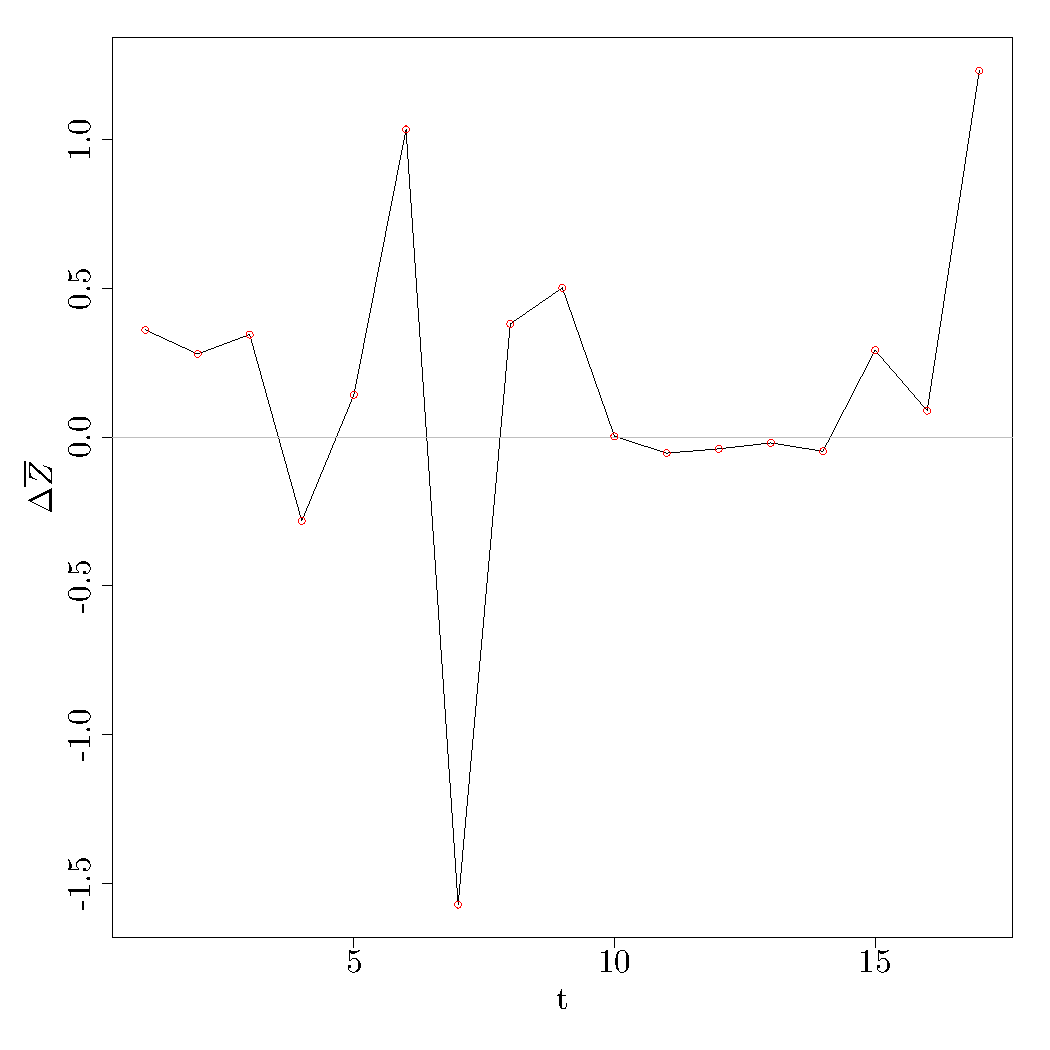
\includegraphics[width=\maxwidth]{figure/decompose_that_stuff} 

\end{knitrout}

So at least the two calculations of $\Delta \overline{Z}$ give consistent results. Now the question is what the different terms contribute to this.
\begin{knitrout}
\definecolor{shadecolor}{rgb}{0.969, 0.969, 0.969}\color{fgcolor}\begin{kframe}
\begin{alltt}
\hlstd{DCs}\hlkwb{<-}\hlstd{(}\hlnum{1}\hlopt{/}\hlstd{Wbar)}\hlopt{*}\hlstd{Zbar}\hlopt{*}\hlstd{Sbar}\hlopt{-}\hlstd{Zbar}
\hlstd{DCr}\hlkwb{<-}\hlstd{(}\hlnum{1}\hlopt{/}\hlstd{Wbar)}\hlopt{*}\hlstd{(Zbar}\hlopt{*}\hlstd{Rbar)}
\hlstd{VS}\hlkwb{<-}\hlstd{(}\hlnum{1}\hlopt{/}\hlstd{Wbar)}\hlopt{*}\hlstd{covZS}
\hlstd{FS}\hlkwb{<-}\hlstd{(}\hlnum{1}\hlopt{/}\hlstd{Wbar)}\hlopt{*}\hlstd{covZR}
\hlstd{Gr}\hlkwb{<-}\hlstd{(}\hlnum{1}\hlopt{/}\hlstd{Wbar)}\hlopt{*}\hlstd{SGbar}
\hlstd{OMD}\hlkwb{<-}\hlstd{Rbar}\hlopt{*}\hlstd{Dbar}\hlopt{/}\hlstd{Wbar}
\hlstd{ODC}\hlkwb{<-}\hlstd{covDR}\hlopt{/}\hlstd{Wbar}
\hlstd{all}\hlkwb{<-}\hlkwd{cbind}\hlstd{(DCs,DCr,VS,FS,Gr,OMD,ODC)}
\hlkwd{par}\hlstd{(}\hlkwc{mar}\hlstd{=}\hlkwd{c}\hlstd{(}\hlnum{6}\hlstd{,}\hlnum{6}\hlstd{,}\hlnum{2}\hlstd{,}\hlnum{2}\hlstd{))}
\hlkwd{plot}\hlstd{(means[range,}\hlnum{1}\hlstd{],means[(range}\hlopt{+}\hlnum{1}\hlstd{),}\hlnum{2}\hlstd{]}\hlopt{-}\hlstd{means[range,}\hlnum{2}\hlstd{],}\hlkwc{type}\hlstd{=}\hlstr{"l"}\hlstd{,}\hlkwc{ylab}\hlstd{=}\hlstr{"$\textbackslash{}\textbackslash{}Delta \textbackslash{}\textbackslash{}overline\{Z\}$"}\hlstd{,}\hlkwc{xlab}\hlstd{=}\hlstr{"t"}\hlstd{,}\hlkwc{ylim}\hlstd{=}\hlkwd{range}\hlstd{(all))}
\hlkwd{abline}\hlstd{(}\hlkwc{h}\hlstd{=}\hlnum{0}\hlstd{,}\hlkwc{col}\hlstd{=}\hlstr{"gray"}\hlstd{)}
\hlkwd{points}\hlstd{(means[range,}\hlnum{1}\hlstd{],overall,}\hlkwc{col}\hlstd{=}\hlstr{'black'}\hlstd{)}
\hlstd{nopoints}\hlkwb{<-}\hlkwd{dim}\hlstd{(all)[}\hlnum{2}\hlstd{]}
\hlstd{cols}\hlkwb{<-}\hlkwd{rainbow}\hlstd{(nopoints)}
\hlkwa{for}\hlstd{(i} \hlkwa{in} \hlnum{1}\hlopt{:}\hlstd{(nopoints))\{}
\hlkwd{lines}\hlstd{(means[range,}\hlnum{1}\hlstd{],all[,i],}\hlkwc{col}\hlstd{=cols[i])}
\hlstd{\}}
\hlkwd{legend}\hlstd{(}\hlstr{"bottomleft"}\hlstd{,}\hlkwc{legend}\hlstd{=}\hlkwd{colnames}\hlstd{(all),}\hlkwc{col}\hlstd{=cols,}\hlkwc{lty}\hlstd{=}\hlnum{1}\hlstd{)}
\end{alltt}
\end{kframe}
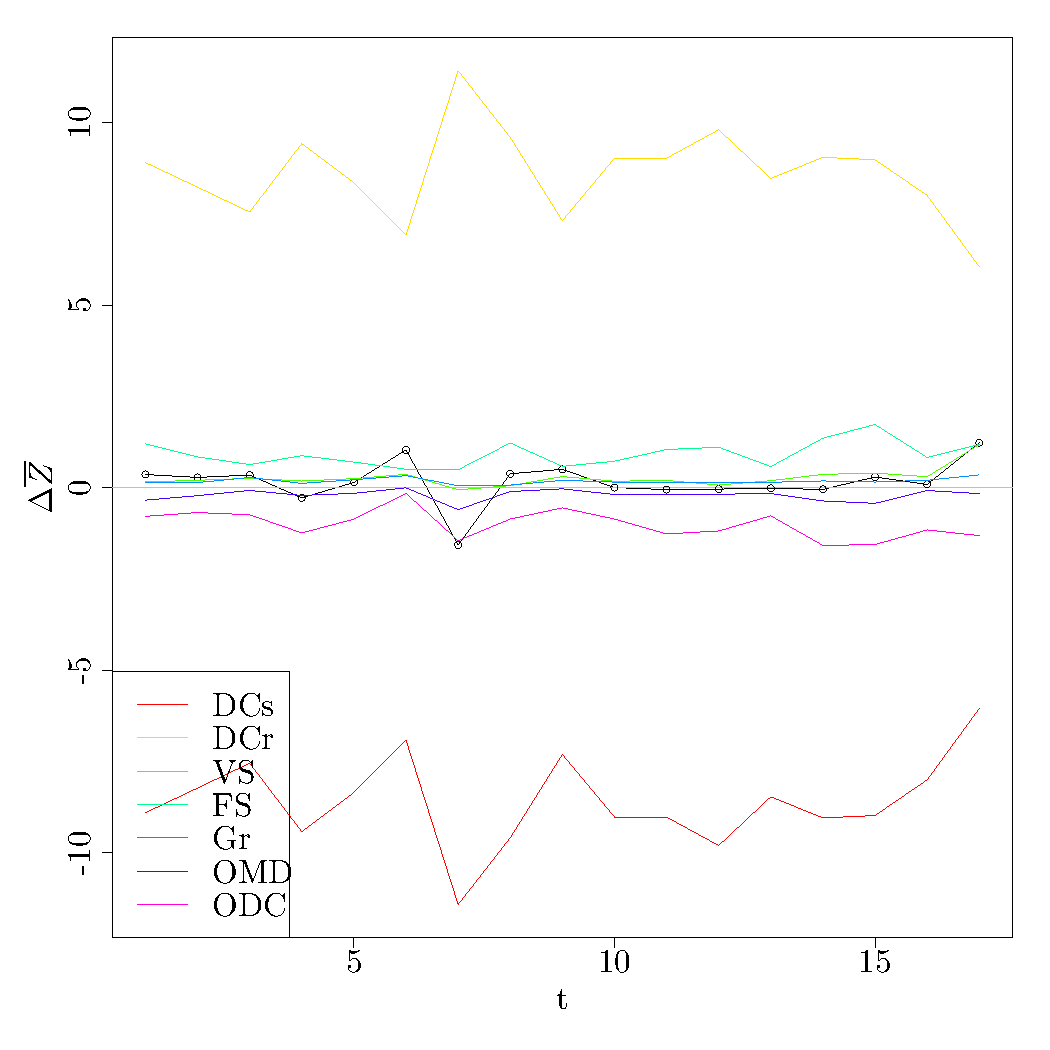
\includegraphics[width=\maxwidth]{figure/moredec} 

\end{knitrout}


\end{document}
